% Generado por scripts/armar_articulo_tex.py desde borrador.md y plantilla.tex.
% No se edita a mano: se cambia el borrador y se vuelve a generar.
% Plantilla del artículo del Proyecto Integrador (Producto de difusión)
% Formato requerido: carta, una columna, 11 pt, márgenes de 2.5 cm, interlineado 1.15.
% Extensión: la rúbrica pide 12 a 18 páginas desde el título hasta las referencias,
% anexos aparte. La plantilla del curso decía aquí «3 páginas», que es la cifra del
% resumen ejecutivo: los dos zips comparten el referencias.bib y el logo byte a byte,
% así que esa línea venía heredada. Manda la rúbrica. Pendiente de confirmar.
% Referencias: APA 7, decidido por el equipo (el resto del proyecto ya cita en APA).
% Compila con pdfLaTeX (opción predeterminada de Overleaf) + Biber.
% Archivos necesarios en la misma carpeta: logo.jpeg, figura_ejemplo.png y referencias.bib
\documentclass[letterpaper,11pt]{article}

% --- Idioma y tipografía ---
\usepackage[T1]{fontenc}
\usepackage{lmodern}
\usepackage[spanish,es-tabla]{babel}

% --- Página: carta, márgenes 2.5 cm, interlineado 1.15 ---
\usepackage[margin=2.5cm]{geometry}
\geometry{headheight=52pt,headsep=0.3cm}
\usepackage{setspace}
\setstretch{1.15}

% --- Figuras y tablas ---
\usepackage{graphicx}
\usepackage{booktabs}
\usepackage{float}
\usepackage[font=small,labelfont=bf,labelsep=colon]{caption}

% --- Encabezado: logo (logo.jpeg) solo en la primera página ---
\usepackage{fancyhdr}
\renewcommand{\headrulewidth}{0pt}
\fancypagestyle{plain}{%
  \fancyhf{}%
  \fancyhead[C]{\includegraphics[height=1.2cm]{logo.jpeg}}%
  \fancyfoot[C]{\thepage}}
\pagestyle{fancy}
\fancyhf{}
\fancyfoot[C]{\thepage}

% --- Cuadros de "Nota de formato" ---
\usepackage[skins,breakable]{tcolorbox}
\newtcolorbox{nota}{%
  enhanced, breakable,
  colback=black!8, colframe=black!8,
  boxrule=0pt, arc=0pt,
  left=3pt, right=3pt, top=2pt, bottom=2pt,
  before skip=10pt, after skip=10pt,
  fontupper=\sffamily\footnotesize\setstretch{1}
}

% --- Encabezados de sección ---
\usepackage{titlesec}
\titleformat{\section}{\Large\bfseries}{\thesection.}{0.6em}{}
\titleformat{\subsection}{\large\bfseries}{\thesubsection.}{0.6em}{}
\titlespacing*{\section}{0pt}{1.6ex plus 0.4ex minus 0.2ex}{1ex}

% --- Referencias: APA 7 ---
\usepackage{csquotes}
\usepackage[style=apa,backend=biber]{biblatex}  % APA 7: decidido, no se cambia a IEEE
\addbibresource{bibliografia.bib}

% --- Enlaces y URL (DOI); se carga al final ---
\usepackage[hidelinks]{hyperref}
\urlstyle{same}

% --- Añadidos para el artículo generado desde borrador.md (scripts/armar_articulo_tex.py) ---
\usepackage{longtable}
\usepackage{array}
\usepackage{calc}
\usepackage{xcolor}
\providecommand{\tightlist}{\setlength{\itemsep}{0pt}\setlength{\parskip}{0pt}}
\addto\captionsspanish{\renewcommand{\tablename}{Tabla}} % babel-spanish dice «Cuadro»; la plantilla pide «Tabla»
\newcounter{none} % el longtable de pandoc declara \LTcaptype{none} y espera que el contador exista
% El campo `note` de bibliografia.bib son anotaciones internas del equipo («LEÍDO PARCIAL», cómo se verificó
% cada entrada): sirven en docs/referencias y no deben salir impresas en las referencias del artículo.
\AtEveryBibitem{\clearfield{note}}
\setlength{\emergencystretch}{3em}
\DeclareUnicodeCharacter{2212}{\ensuremath{-}}
\DeclareUnicodeCharacter{2265}{\ensuremath{\geq}}
\DeclareUnicodeCharacter{2192}{\ensuremath{\rightarrow}}
\DeclareUnicodeCharacter{00B5}{\ensuremath{\mu}}

% --- Título ---
\title{\textbf{Qué mueve el resultado al predecir la actividad de compuestos naturales}}
\author{Ingrid Pamela Ruiz Puga\quad Artemio Santiago Padilla Robles\\[2pt] José Antonio Vázquez Martínez\\[6pt]
  \normalsize Proyecto Integrador · Maestría en Inteligencia Artificial Aplicada \\[6pt]
  \normalsize Asesora: Dra. Grettel Barceló Alonso \quad·\quad Patrocinadora: Dra. Mariana Martínez Ávila \\[2pt]
  \normalsize 13 de noviembre de 2026}
\date{\vspace{-2ex}}

\begin{document}

\maketitle

\begin{abstract}
Buscamos compuestos naturales con potencial neuroprotector con dos modelos en paralelo: uno que clasifica si una molécula cruza la barrera hematoencefálica (fase 1) y otro que predice su potencia contra una diana, usando también las mediciones censuradas (fase 2). Comparamos once modelos y ningún ensamble mejora de forma distinguible al mejor modelo individual en MCC ni en AUPRC; en AUROC dos ensambles lo superan por 1.3 puntos, diferencia que no sobrevive a la corrección por diez comparaciones. Lo que sí mueve el resultado es una lección conocida \autocite{sheridan2013,roberts2017crossvalidation}, medida aquí con sus magnitudes: \textbf{cuánta semejanza se permite entre lo que se entrena y lo que se evalúa}. Con el modelo que entregamos, el MCC baja 33.3 puntos al exigir que ningún compuesto de entrenamiento se parezca más de 0.4 a uno de validación, contra 4.2 puntos entre los once modelos; la fase 2 muestra la misma escalera. Tres hallazgos propios: la prueba reservada es \textbf{más difícil de lo que su similitud predice} (AUROC esperado 0.89, observado 0.79); el MCC exagera esa caída porque corta en un punto fijo; y las huellas moleculares ayudan en la fase 2 y no en la 1, sin que lo expliquen el tamaño de los datos ni el tipo de etiqueta. El modelo de potencia, elegido por funcionar en compuestos que solo existen en NPASS, no se sostiene en la prueba en ese grupo (117 pares).
\end{abstract}

\begin{figure}[H]
  \centering
  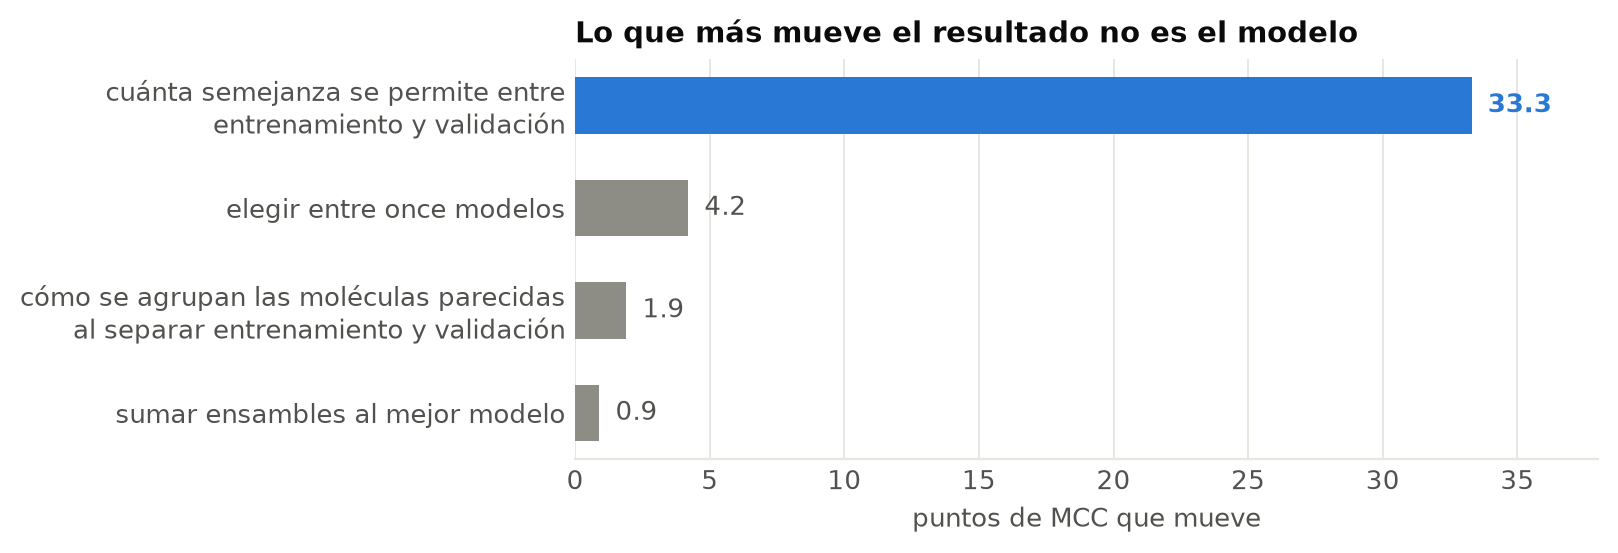
\includegraphics[width=0.9\linewidth]{figuras/f0_palancas.png}
  \caption{Cada barra viene de una corrida distinta, con otro propósito; indican el orden de magnitud, no miden el efecto de cada factor por separado.}
  \label{fig:f0_palancas}
\end{figure}

\section{Contexto de negocio y problema}
La patrocinadora, del Departamento de Bioingeniería del Tec de Monterrey, busca priorizar compuestos naturales con potencial neuroprotector y nootrópico antes de ensayarlos en el laboratorio, donde cada ensayo gasta tiempo y presupuesto. Un compuesto natural bioactivo solo sirve si llega al cerebro y si actúa sobre una diana, así que el problema tiene dos preguntas: si la molécula cruza la barrera hematoencefálica (fase 1, clasificación BBB+/BBB−) y con qué potencia actúa sobre cada una de 26 dianas del sistema nervioso central (fase 2, regresión). La entrada es la estructura (SMILES) y la salida es una lista priorizada, no una decisión automática.

\textbf{El enfoque que se adoptó.} El planteamiento inicial encadenaba las dos preguntas: lo que saliera BBB− se descartaba. Se abandonó porque esa predicción no está verificada para la mayoría de los compuestos: solo 1,033 esqueletos tienen medición en los dos conjuntos, y el otro 99\% se filtraría con una predicción no comprobada. Los dos modelos son, por eso, evidencia paralela que se combinará en un ranking y no una cascada (la combinación sigue pendiente, decisión C.3).

\textbf{Qué significa equivocarse.} Un falso permeable manda al laboratorio a ensayar algo que no funciona; un falso no permeable descarta un candidato real sin que nadie se entere. Cuál error cuesta más lo decide el laboratorio, y por eso el entregable es un orden y no un punto de corte (decisión C.5).

\section{Datos y preparación}
\begin{itemize}
\tightlist
\item
  \textbf{Fase 1 (permeabilidad).} 7,805 compuestos con clase, del archivo curado de la patrocinadora (derivado de B3DB y cruzado con COCONUT, lo que permite separar los naturales de los sintéticos); 65\% BBB+; 6,306 para ajustar y validar y 1,499 reservados. No se filtra por la columna de grupo de confiabilidad (A a D): el análisis exploratorio mostró que está confundida con la clase, y filtrar empeora el desbalance en vez de limpiar ruido.
\item
  \textbf{Fase 2 (potencia).} 202,647 registros de actividad (ChEMBL, NPASS, CMAUP); 56,241 pares para ajustar y 13,944 reservados. Las tres fuentes se etiquetan con las mismas columnas, porque la medida que solo trae ChEMBL descartaría justo los naturales de NPASS y CMAUP. Se guarda el intervalo de potencia y no una etiqueta, porque el corte de 10 µM, heredado del cribado, es una decisión que puede cambiar y porque el mismo compuesto cambia de clase según la concentración. Los resultados se reportan por procedencia: un modelo que solo ve de dónde viene un compuesto ya alcanza 65\% del MCC de la química.
\item
  \textbf{Variables.} Descriptores 2D de RDKit (151 tras quitar los casi constantes y los redundantes, con la selección hecha sobre valores crudos) y, en la fase 2, la diana. Las huellas moleculares se midieron aparte (sección 4.4).
\item
  \textbf{Partición.} Nunca al azar: se agrupa por andamio de Bemis--Murcko \emph{unido} al esqueleto de conectividad, para que los estereoisómeros no caigan a los dos lados (1,048 grupos en la fase 1).
\end{itemize}

\section{Metodología y modelos}
\textbf{Del baseline al modelo final.} \emph{Baseline} (Avance 3): tres canalizaciones con validación cruzada agrupada, 3 semillas × 5 pliegues: boosting por histogramas, bosque aleatorio y regresión logística (MCC 0.702, 0.700 y 0.687; los intervalos del 95\% se solapan y ninguna gana). Su resultado fijó el desempeño mínimo que había que superar, \textbf{0.70 de MCC} (y 0.93 de AUROC), contra un piso de 0 de MCC, 0.5 de AUROC y 0.35 de AUPRC que dan los clasificadores triviales. \emph{Candidatos} (Avances 4 y 5): once modelos de clasificación, de la regresión logística a cinco ensambles y dos versiones afinadas, con una regla de mejora escrita antes de correr: una diferencia pareada media por encima de un umbral y positiva en al menos 12 de las 15 evaluaciones. \emph{Modelo final:} ninguna de las treinta comparaciones contra el mejor individual pasó la regla, así que el final de la fase 1 es ese mejor individual, \texttt{svm\_rbf} sobre 151 descriptores; se eligió por descarte y no porque ganara. En la fase 2, tras comparar nueve modelos de regresión, el final es un modelo de supervivencia acelerada (AFT, XGBoost \autocite{chen2016xgboost}) que aprende de las mediciones censuradas.

\textbf{Rigor.} Las reglas de decisión se escribieron antes de cada corrida y no se ajustaron después (no están pre-registradas); cada corrida reproduce una cifra ya registrada como control, y cada resultado nuevo se recalculó con un segundo código. Los intervalos remuestrean grupos, no filas. De los seis modelos de la fase 1, cuatro (incluido el entregado) dan la misma predicción con cualquier semilla; el \texttt{mlp} y el \texttt{bosque} no (desviación de 0.017 y 0.007 de MCC). La prueba reservada se leyó \textbf{catorce veces}, cuatro de ellas sin etiquetas ---dos solo como SMILES (la escalera ampliada y la distribución de similitud de la prueba) y dos solo estructurales (la proporción de andamios, una por fase)---, todas registradas en \texttt{experimentos/prueba.csv}; ningún modelo se eligió después de verla. Las dos de la 1.11 reparten la prueba entre ajuste y evaluación, reajustan el modelo y lo evalúan con etiquetas sobre el núcleo de evaluación en 15 sorteos, sin reevaluar el modelo final entregado; la última (C.5, \#191) lee el MCC del modelo final a cuatro cortes, con el corte elegido y congelado en validación antes de leerla.

\textbf{Métricas.} El AUROC mide qué tan bien el modelo ordena a los compuestos permeables por encima de los no permeables, sin fijar un corte. El MCC (coeficiente de correlación de Matthews) resume en un número entre −1 y 1 las cuatro casillas de la matriz de confusión y \textbf{sí exige un corte}, aquí 0.5; por eso se mueve más que el AUROC cuando cambia la distribución de los datos. El AUPRC sobre la clase minoritaria se lee contra su tasa base (0.35 en la fase 1), no contra cero. En la fase 2, donde la respuesta es una potencia con mediciones censuradas, se usa la concordancia de Harrell: la probabilidad de que, de dos pares, el modelo ordene bien al más potente (0.5 es el azar). Los modelos se comparan con la diferencia pareada en las mismas 15 evaluaciones (3 semillas × 5 pliegues), con el intervalo corregido de Nadeau y Bengio \autocite{nadeau2003inference}.

\section{Resultados y validación}
\subsection{El modelo final contra el baseline y el umbral}

Contra el umbral de 0.70 de MCC que fijó el baseline, el modelo entregado lo iguala en validación cruzada y no lo supera: MCC 0.7017 (el boosting del baseline daba 0.7019), AUROC 0.919 y AUPRC de la clase minoritaria 0.884, contra un piso de 0.35. \textbf{El lift sobre el baseline es cero}, y es un resultado: elegir el modelo no fue la palanca. En la prueba reservada, leída una sola vez con el modelo final, el MCC es 0.339, el AUROC 0.793 y el AUPRC 0.720: una \textbf{brecha de 0.363 de MCC (52\%) y de 0.126 de AUROC (14\%)} frente a la validación cruzada. En la fase 2 la concordancia baja de 0.761 a 0.720. El AUROC de 0.93 del baseline sale de predicciones promediadas entre semillas y no se compara con el 0.919, que es el promedio de las 15 evaluaciones.

\textbf{Qué significan los errores para el laboratorio.} A 0.5 el modelo declara permeable al 70.9\% de los compuestos cuando la prevalencia real es 64.97\%: de más, que es el error que gasta un ensayo. Pero la caída del MCC es mayor que la del AUROC porque el MCC exige un corte fijo y, bajo un cambio de distribución, el modelo cambia de sesgo (sección 4.2). Por eso el cuaderno entrega la probabilidad y no una clase, y lo que el laboratorio debe leer es el orden.

\subsection{La escalera de semejanza}

Entre los once modelos hay 4.2 puntos de MCC. Con el \texttt{svm\_rbf}, pasar de pliegues al azar a pliegues donde ningún compuesto de entrenamiento supera 0.4 de similitud con uno de validación cuesta 33.3 puntos (0.752 → 0.419). En validación cruzada, el modelo entregado da MCC 0.702 y AUROC 0.919.

\begin{figure}[H]
  \centering
  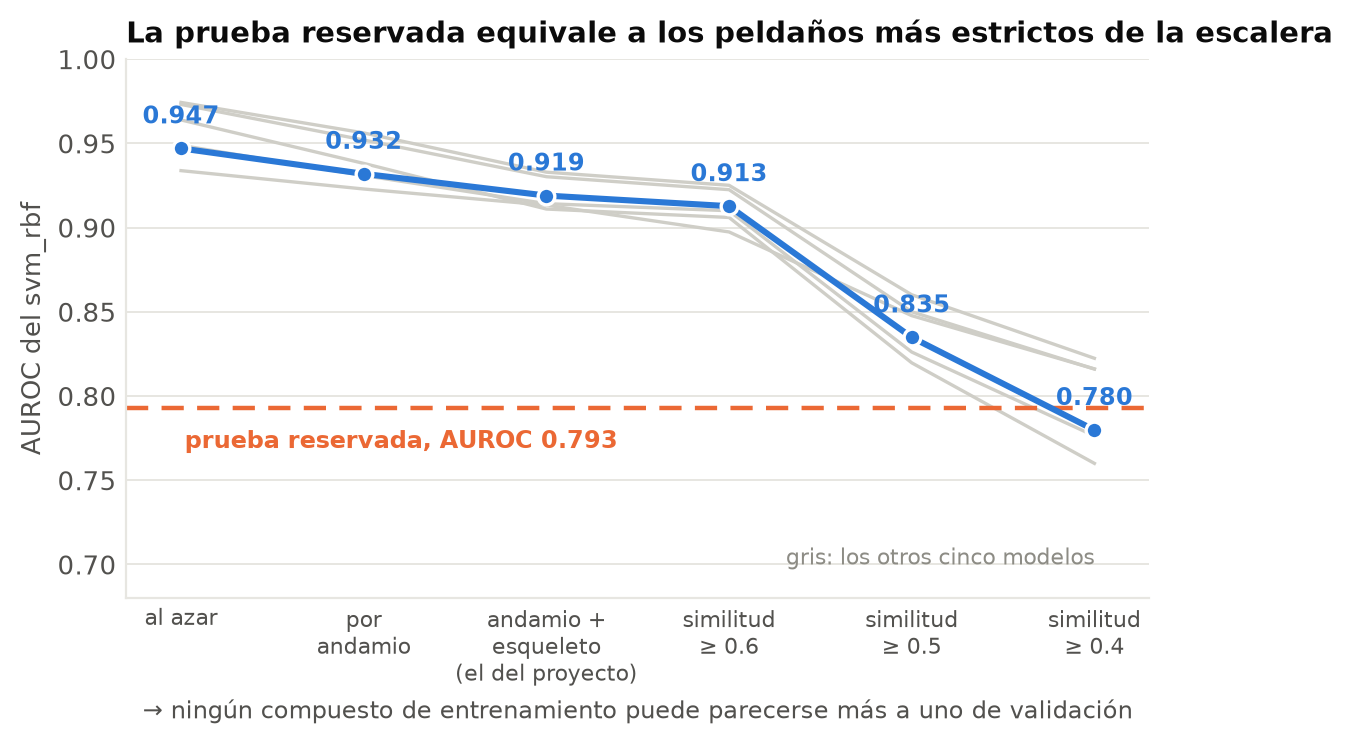
\includegraphics[width=0.9\linewidth]{figuras/f1_escalera.png}
  \caption{AUROC por peldaño, seis modelos. La línea naranja es la prueba reservada (0.793).}
  \label{fig:f1_escalera}
\end{figure}

\textbf{La fase 2 muestra lo mismo, con una limitación del conjunto.} La concordancia del \texttt{aft} baja de 0.807 (por molécula) a 0.695 con similitud ≥ 0.6, siete veces la dispersión entre los modelos competitivos. A 0.5 y 0.4 no se puede ni construir la partición: el 69\% y el 90\% de las filas caen en un solo grupo. No hay manera de evaluar la fase 2 con química realmente nueva a esos niveles.

\begin{figure}[H]
  \centering
  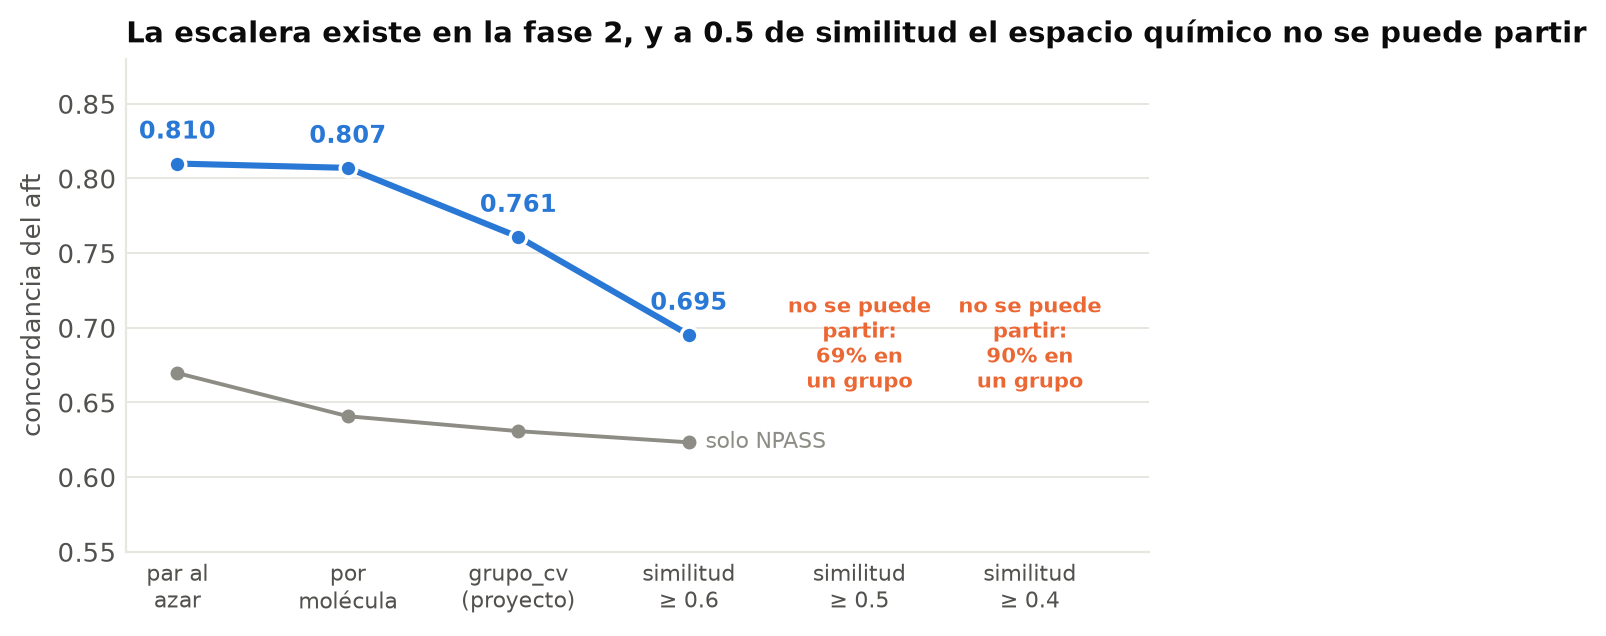
\includegraphics[width=0.9\linewidth]{figuras/f6_escalera_fase2.png}
  \caption{Concordancia del \texttt{aft} por peldaño; en gris, solo pares de NPASS.}
  \label{fig:f6_escalera_fase2}
\end{figure}

\textbf{Dos matices que el artículo tiene que llevar.} La \emph{forma} de la escalera depende de cómo se defina «parecido»: con ECFP6 la caída es gradual y con ECFP4 casi todo ocurre entre 0.6 y 0.5, aunque la caída total es parecida (0.419 contra 0.434 de MCC); con atom-pair no se pueden construir los peldaños estrictos. Y el MCC exagera: con el mejor corte posible sería 0.655 y 0.560 en los dos peldaños estrictos, contra 0.486 y 0.419 con el corte fijo en 0.5. Un corte de igual prevalencia solo recupera +0.047 en el primero, así que no es una solución.

\subsection{La prueba reservada es más difícil de lo que su similitud predice}

En la prueba el AUROC es 0.793 y el MCC 0.339 (1,499 compuestos). Su similitud media al vecino más cercano (0.414) es mayor que la de la validación agrupada (0.384), así que por similitud tendría que rendir \emph{mejor}: reponderar las predicciones de validación a su distribución de similitud da un AUROC esperado de \textbf{0.89}, y el real es \textbf{0.79}. La brecha de 0.10 no se explica por qué tan lejos queda de lo visto; qué es, no está medido (candidatos: prevalencia, peso y polaridad, curación de los datos, andamios raros a propósito).

Dentro de la prueba, la ventaja del modelo sobre una línea base de peso molecular y TPSA crece con lo parecido que es cada compuesto (+0.036 en el tercil más raro, +0.106 en el más parecido; diferencia +0.069, IC95\% 0.011 a 0.124); en la fase 2 la diferencia es cuatro veces menor.

\textbf{La caída baja con la similitud.} Dividiendo la prueba en terciles de similitud al ajuste (cortes 0.31 y 0.46), el AUROC sube de 0.697 a 0.793 y a 0.875: +0.178 entre el tercil más parecido y el menos parecido, IC95\% {[}+0.119, +0.238{]} remuestreando esqueletos. En los compuestos sin equivalente natural la diferencia es +0.223 {[}+0.142, +0.306{]}; en los naturales exactos es +0.086 con un intervalo que incluye el cero {[}−0.029, +0.204{]}, así que con 446 compuestos no se distingue, y en los análogos estereoquímicos el tercil más parecido tiene menos de 20 casos de la minoritaria y no se reporta. Es una correlación dentro de la prueba y la similitud no explica toda la brecha (0.89 esperado contra 0.79).

\begin{figure}[H]
  \centering
  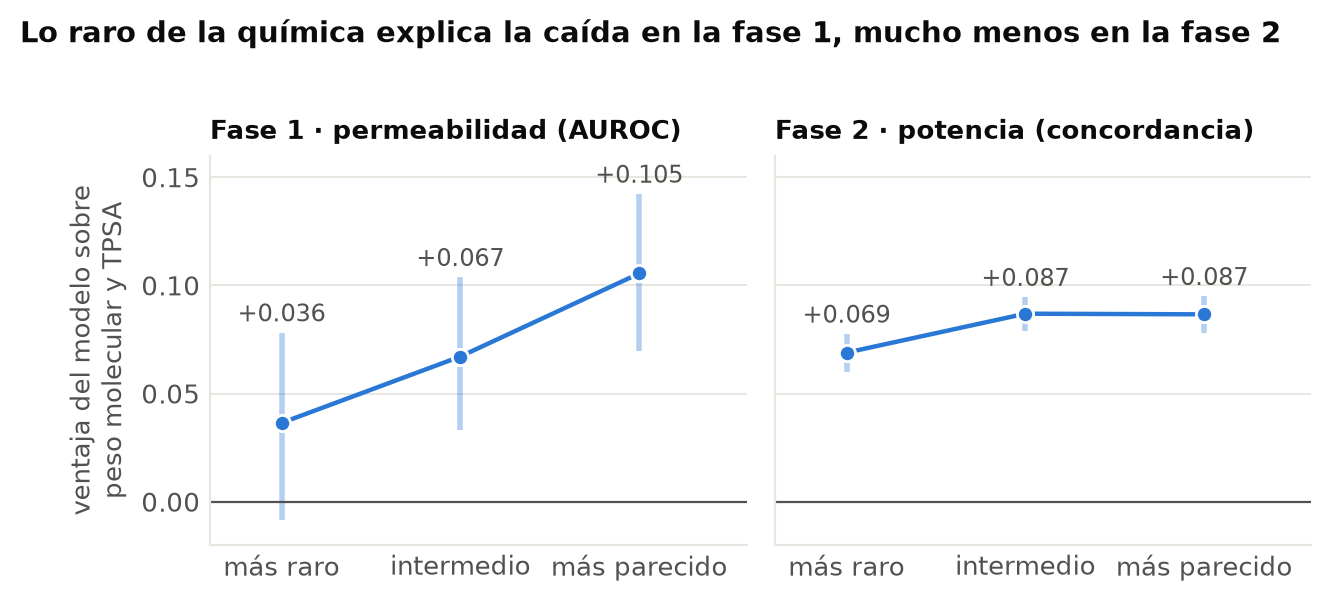
\includegraphics[width=0.9\linewidth]{figuras/f2_rareza.png}
  \caption{Ventaja sobre la línea base por tercil de rareza, con IC95\% por bootstrap de grupos.}
  \label{fig:f2_rareza}
\end{figure}

\textbf{Dar más peso a lo raro durante el entrenamiento no ayuda.} Como la ventaja del modelo se pierde justo en lo raro, probamos repesar las filas raras que ya están en el ajuste: peso 3, 2 y 1 según el tercil de similitud al vecino más cercano de otro grupo, dentro de cada tramo de peso molecular (\texttt{svm\_rbf}, 15 evaluaciones agrupadas, regla escrita antes de correr, sin leer la prueba; decisión 1.10). En el tercil más raro de validación la ganancia de AUROC es −0.0005, positiva en 9 de 15 evaluaciones, cuando la regla pedía más de 0.005 en 12. Un control con los mismos pesos asignados al azar mueve el AUROC global casi igual (+0.0015 contra +0.0022) y el MCC global baja 0.0022. \textbf{La regla tiene poca potencia para efectos chicos:} con la dispersión observada (0.0095) solo detectaría con 80\% de probabilidad una mejora de unos 0.010, así que el resultado descarta una mejora grande, no una de 0.005.

\textbf{Pasar compuestos raros de la prueba al entrenamiento tampoco cierra la brecha.} Probamos la otra forma de aprender de lo raro (decisión 1.11, la lectura 12 de la prueba, regla escrita antes de correr). La mitad de los grupos de la prueba de cada tercil de rareza forma un núcleo de evaluación; de la otra mitad se pasan al ajuste las filas del tercil más raro (285 de media) y se devuelven a la prueba otras tantas filas comunes del ajuste, en 15 sorteos. En lo raro del núcleo el AUROC sube +0.003 (mejor en 9 de 15), y pasar el mismo número de filas de la prueba \textbf{elegidas al azar} da +0.006: lo que ayuda es recibir filas de la prueba, no cuáles. El MCC pasa de 0.33 a 0.36 (+0.035, en los 15 sorteos), lejos del 0.70 de la validación, mientras el AUROC apenas cambia (+0.002) y el azar también lo sube: el orden casi no cambia y el corte sí, así que no lo leemos como ganancia. No lo explica la prevalencia del entrenamiento, que casi no se mueve (de 65.0\% a 64.5\% de BBB+). Lo más útil de la corrida es otra cosa: los compuestos comunes que pasan a la prueba se miden con AUROC 0.94 y los raros que quedaban en 0.68, con el mismo modelo y sin reentrenar; recomponer la prueba cambia el número que se reporta y no lo que el modelo sabe. Los 15 sorteos comparten las mismas 1,499 filas, así que el resultado descarta una ganancia grande y no una pequeña. No se adopta nada: 285 filas más de química rara no cierran la brecha entre 0.70 y 0.34 de MCC.

\textbf{Recomponer con cuáles filas se entrena tampoco ayuda.} La tercera forma (decisión 1.12) fija el tamaño, la prevalencia y el número de grupos del ajuste y cambia solo su composición. Empezar por lo raro cuesta −0.060 de AUROC contra el orden al azar con el 25\% del ajuste (IC95\% {[}−0.110, −0.011{]}, a favor en 1 de 15 evaluaciones; es una comparación secundaria, declarada antes y sin corrección por comparaciones múltiples, y el estadístico principal incluye el cero); con el 75\% la composición deja de importar (±0.0004), y ni siquiera mejora el tercil más raro de la validación (+0.003, 8 de 15). \textbf{Ninguna de las formas que probamos de aprender de lo raro ---repesar, pasar filas de la prueba al ajuste y recomponer--- cierra la brecha}, y añadir filas al azar ya estaba en meseta en la curva de aprendizaje. El límite de la fase 1 no es de cuántas filas ni de cuáles; lo que queda por medir es el punto de operación.

\textbf{El punto de operación sí mueve el MCC, pero no se elige con validación.} A 0.5 el modelo entregado declara permeable al 79.3\% de la prueba contra una prevalencia real de 57.3\%: 22 puntos de desajuste, contra 6 en el ajuste (decisión C.5, lectura 14 de la prueba). Un corte elegido en validación interna agrupada, congelado antes de leerla, no recupera nada (MCC 0.3455 contra 0.3385; diferencia +0.0065, IC95\% {[}−0.022, +0.034{]}), porque se elige donde la prevalencia es 65.0\% y no puede saber que la de llegada es otra. Igualar la tasa declarada a una prevalencia supuesta (aquí la del ajuste, 65.0\%) sube el MCC a 0.4095 (+0.071, IC95\% {[}+0.030, +0.110{]}), casi la mitad del margen que deja el corte óptimo de la prueba (0.485), que usa sus etiquetas. Exige tener el lote completo y suponer una prevalencia; con el AUROC igual (0.793), el MCC dice cuánto cambió la tasa de aciertos de un punto de corte y no la capacidad de ordenar.

\subsection{La representación no se traslada entre fases}

Las huellas Sort \& Slice \textbf{no mejoran a ningún modelo de la fase 1} y bajan el MCC de cinco de seis; en la fase 2 mejoran a cinco de seis en las 15 evaluaciones. Por tramo de peso la media es negativa en la fase 1 sin tendencia y crece con el peso en la fase 2.

El detalle por tramo de peso está en el Anexo C.

Dos explicaciones simples se \textbf{descartaron} con experimentos propios. \textbf{No es el tamaño de los datos}: con el ajuste de la fase 2 reducido a 5,000 filas (el de la fase 1) la ganancia del \texttt{aft} es +0.0105 en 14 de 15 evaluaciones, mayor que con el ajuste completo (+0.0057). \textbf{No es la granularidad de la etiqueta}: con la etiqueta «molécula activa contra alguna diana» las huellas ayudan a los cuatro modelos probados (AUROC +0.017 a +0.085).

\begin{figure}[H]
  \centering
  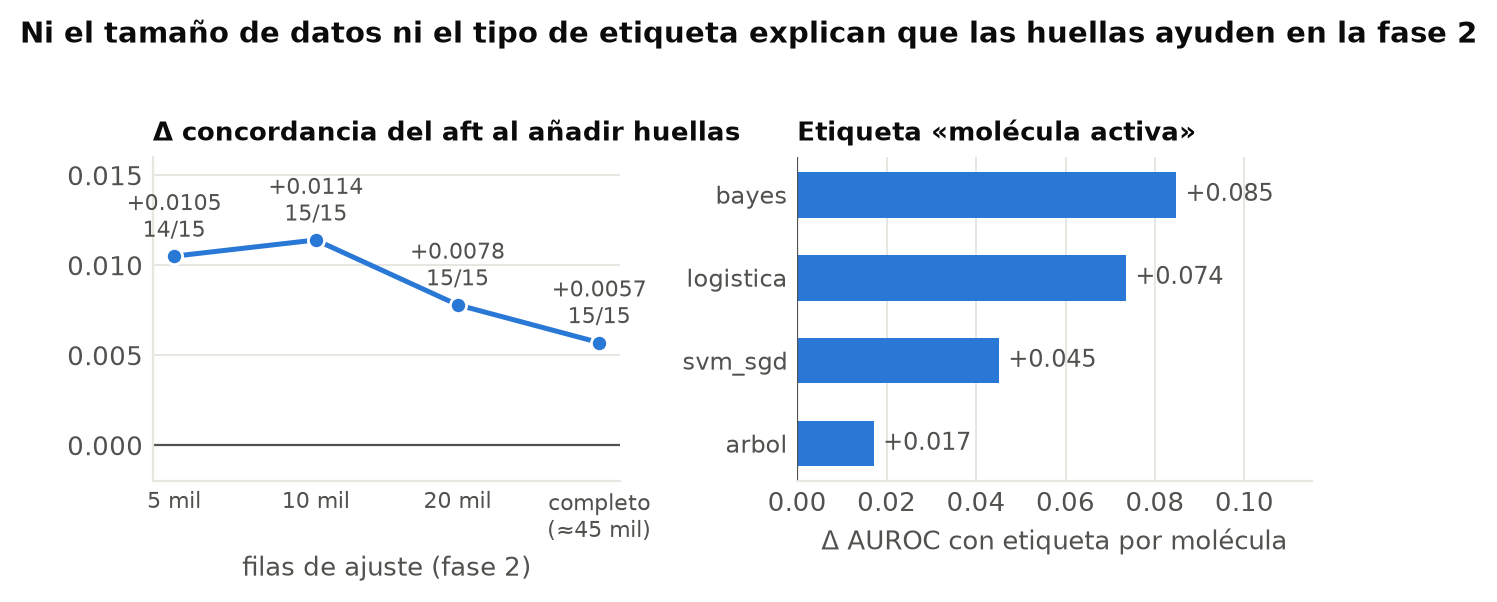
\includegraphics[width=0.9\linewidth]{figuras/f5_rivales.png}
  \caption{Las huellas ayudan aunque se achiquen los datos o se cambie la etiqueta.}
  \label{fig:f5_rivales}
\end{figure}

Quedan en pie dos hipótesis. \textbf{La densidad del espacio químico} (que las huellas ganen donde hay muchos vecinos) se midió a igual peso molecular y el resultado es \textbf{no concluyente}: la fase 2 es 1.8 veces más densa que la 1 (61.9 contra 33.8 vecinos fuera del grupo), y en la fase 1 la pérdida por añadir huellas se concentra en el tercio más disperso, pero las diferencias no superan su desviación. Y que \textbf{la permeabilidad dependa de propiedades globales} que los descriptores ya capturan mientras la unión depende de subestructuras: no está medida. Los resultados valen para esas familias de modelos y no prueban qué pasa en la fase 1.

\subsection{El modelo de potencia en NPASS}

El AFT se eligió porque en los pares que solo tiene NPASS aprende de mediciones censuradas que los demás descartan. En validación cruzada su concordancia ahí es 0.632 contra 0.511 del bosque. En la prueba (117 pares) baja a 0.530 en la corrida registrada (0.511 al reajustarlo, que es lo que muestra la figura) y la línea base de peso y TPSA da 0.565. Con 117 pares no hay potencia para distinguir 0.511 de 0.632, y los pares no son la misma población (12.3\% de activos contra 44.4\%): \textbf{no refuta el resultado, pero tampoco lo confirma.} Además, su ventaja de MCC sobre el bosque (+0.155 con corte fijo) se reduce a +0.028 con un corte de igual prevalencia; sigue siendo positiva en las 15 evaluaciones y coincide con su ventaja de AUROC (+0.012).

\begin{figure}[H]
  \centering
  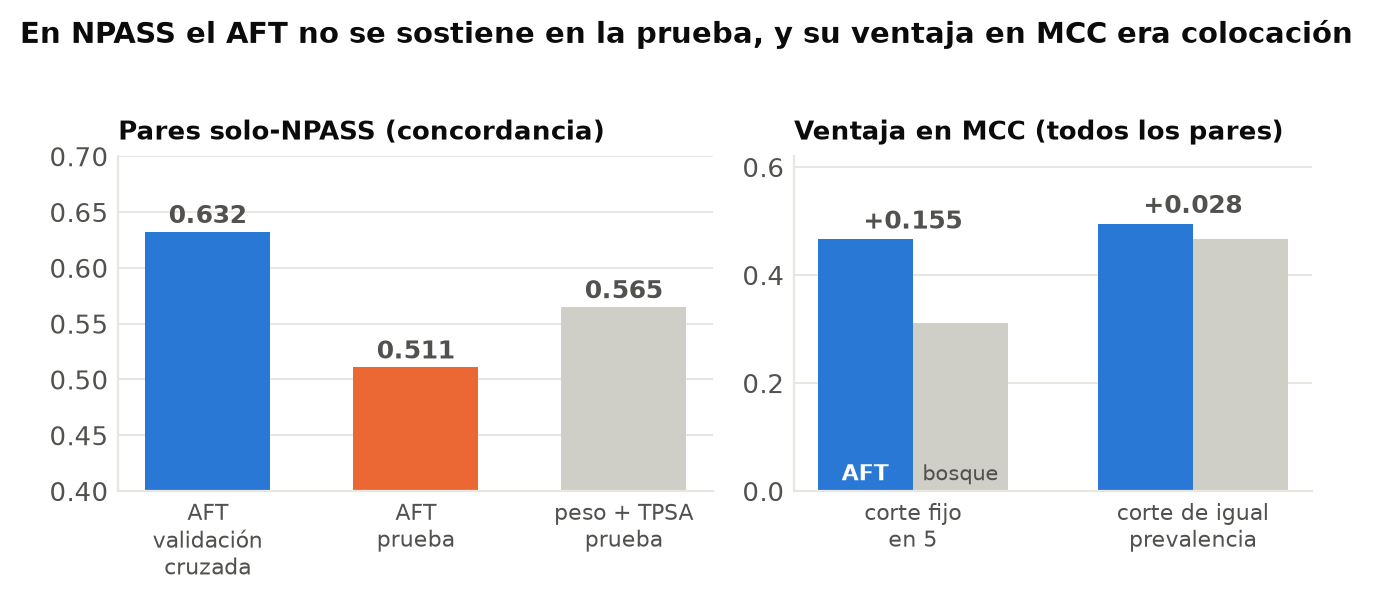
\includegraphics[width=0.9\linewidth]{figuras/f4_aft.png}
  \caption{Izquierda: concordancia solo-NPASS. Derecha: ventaja en MCC del AFT sobre el bosque.}
  \label{fig:f4_aft}
\end{figure}

Ningún otro brazo supera al \texttt{aft} en NPASS (filtrar los descriptores no cambia nada y quitarlos lo empeora 0.041), y dos métodos de atribución independientes concuerdan en lo que pesa, con la diana en primer plano y TPSA y los donadores de hidrógeno lejos (Anexo F).

\emph{La operación de estos modelos ---un cuaderno, no un servicio--- está en la sección 5.}

\section{Implementación y operación}
\textbf{Qué se entrega: un cuaderno, no un servicio.} En la reunión del 3 de noviembre la patrocinadora dijo que no habrá un punto de acceso productivo; lo que conviene es dejarle un cuaderno que ella ejecute con sus propios compuestos. La entrada es una lista de SMILES; la salida, para cada compuesto, la probabilidad de cruzar la barrera (fase 1), la potencia predicha contra cada una de las 26 dianas (fase 2, una pActividad por diana y sin intervalo) y qué tan cerca queda de lo que los modelos vieron. \textbf{El cuaderno no combina las dos fases en un ranking}: esa combinación sigue pendiente (decisión C.3), y cuando exista será evidencia paralela y \textbf{no una cascada}, porque un BBB− no descarta un compuesto.

\textbf{Estado hoy.} Los dos modelos finales están guardados en \texttt{models/finales/} (unos 3 MB), con un módulo de inferencia que no necesita los datos de entrenamiento, un script que los regenera y el cuaderno que los usa (\texttt{notebooks/\allowbreak{}06\_\allowbreak{}Uso\_\allowbreak{}de\_\allowbreak{}los\_\allowbreak{}modelos.ipynb}, \#261). Está comprobado que los descriptores calculados desde un SMILES coinciden bit a bit con los de entrenamiento (150 moléculas de cada fase) y que el modelo recargado reproduce al entrenado. Falta que el equipo los revise. El reajuste de la fase 2 con las filas de ajuste no reproduce exactamente la cifra de la prueba (0.7234 contra 0.7200). \textbf{Con qué filas se entrenan} lo decide la curva de aprendizaje y la decisión del 4 de noviembre: \textbf{los dos modelos se sirven con las filas de ajuste}. En la fase 1 la ganancia de usar el 100\% sobre el 75\% es +0.002 de AUROC (meseta); en la fase 2 sigue subiendo (+0.0076 de concordancia en 15 de 15), y se renuncia a esa ganancia a cambio de poder evaluar y repetir la cifra registrada.

\begin{figure}[H]
  \centering
  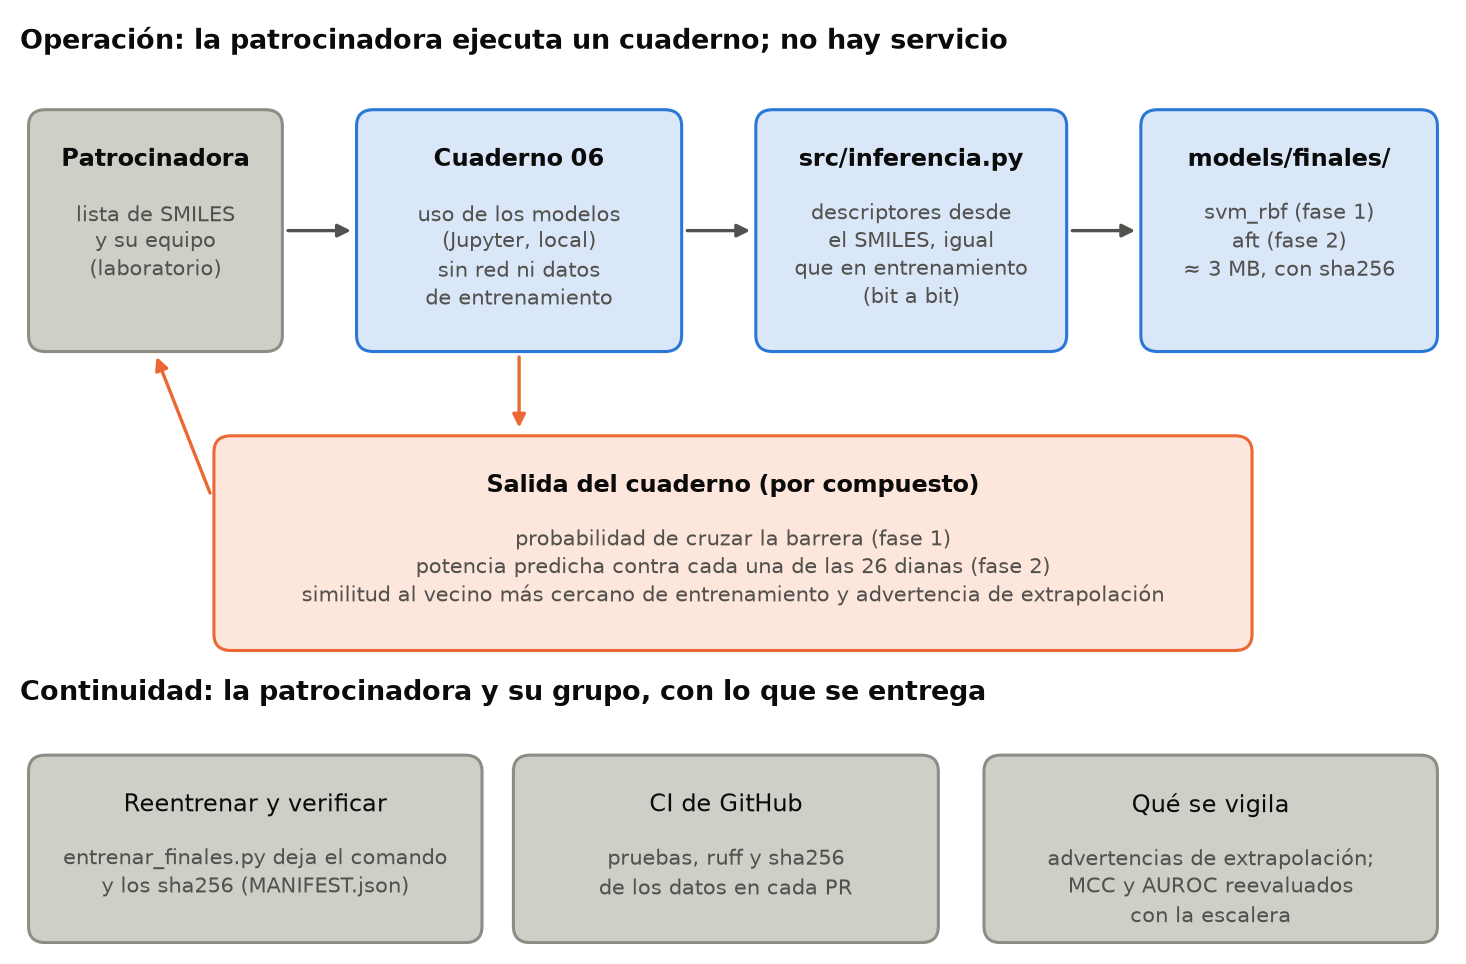
\includegraphics[width=0.9\linewidth]{figuras/f7_despliegue.png}
  \caption{Arquitectura de despliegue: la patrocinadora ejecuta un cuaderno local que llama a un módulo de inferencia y a dos modelos guardados; no hay servicio. Abajo, lo que mantiene el equipo.}
  \label{fig:f7_despliegue}
\end{figure}

La Tabla 1 lista los requisitos para operar y quién responde de cada uno.

\begin{longtable}[]{@{}
  >{\raggedright\arraybackslash}p{(\linewidth - 4\tabcolsep) * \real{0.2564}}
  >{\raggedright\arraybackslash}p{(\linewidth - 4\tabcolsep) * \real{0.3077}}
  >{\raggedright\arraybackslash}p{(\linewidth - 4\tabcolsep) * \real{0.4359}}@{}}
\caption{Requisitos para operar los modelos, por qué se piden y quién responde de cada uno. «Por revisar» indica lo que el equipo aún no ha revisado.}\tabularnewline
\toprule\noalign{}
\begin{minipage}[b]{\linewidth}\raggedright
requisito
\end{minipage} & \begin{minipage}[b]{\linewidth}\raggedright
por qué
\end{minipage} & \begin{minipage}[b]{\linewidth}\raggedright
responsable
\end{minipage} \\
\midrule\noalign{}
\endfirsthead
\toprule\noalign{}
\begin{minipage}[b]{\linewidth}\raggedright
requisito
\end{minipage} & \begin{minipage}[b]{\linewidth}\raggedright
por qué
\end{minipage} & \begin{minipage}[b]{\linewidth}\raggedright
responsable
\end{minipage} \\
\midrule\noalign{}
\endhead
\bottomrule\noalign{}
\endlastfoot
script que entrena y guarda los dos modelos finales, con el comando y los \texttt{sha256} de los datos & que cualquiera pueda reconstruirlos (\texttt{experimentos/README.md} ya lo hace para las corridas) & hecho (\#261), por revisar \\
cuaderno de uso con SMILES propios & es la forma de operación acordada & hecho (\#261), por revisar \\
\textbf{advertencia de extrapolación}: la similitud de cada compuesto consultado a su vecino más cercano de entrenamiento & una cifra de validación cruzada no describe a la química nueva; la escalera de la sección 4.2 muestra cuánto & hecho en el cuaderno (\#261), por revisar \\
reentrenar al llegar datos nuevos y \textbf{reevaluar con la escalera}, no con un corte al azar & evita celebrar una cifra inflada & patrocinadora, con apoyo del equipo \\
evaluación externa con su conjunto de prueba & la prueba reservada es nuestra, no la de ella & \textbf{hecha una vez} con el \texttt{aft} final: concordancia 0.792 {[}0.787, 0.797{]} en 8,134 pares (\texttt{solo\_npass} 0.667, 249 pares), pero \textbf{no comparable}: el 64.9\% de sus pares tiene andamio ya visto; ver abajo \\
\end{longtable}

\textbf{La base externa de la patrocinadora (4 nov).} El archivo \texttt{Testeo} no comparte identificador ni SMILES canónico con el de entrenamiento. Con el \texttt{aft} guardado, sin reentrenar, la concordancia en 8,134 pares de las 26 dianas del modelo es \textbf{0.792} (IC95\% remuestreando esqueletos: 0.787 a 0.797), mayor que el 0.720 de la prueba reservada; en \texttt{solo\_chembl} 0.786, en \texttt{mixto} 0.615 y en \texttt{solo\_npass} 0.667 (249 pares, Spearman 0.309). \textbf{Esa base no es comparable con la prueba reservada:} se separó por compuesto y no por andamio, y el 64.9\% de sus pares tiene un andamio que ya está en el ajuste (contra 0.5\% en el control interno), con una similitud mediana al vecino más cercano de 0.787 (0.679 en la validación de la misma fase). Que salga mejor es lo que predice la tesis del artículo, no una prueba de mejor generalización. Los naturales siguen siendo el estrato débil. Es una lectura única; el control reconstruye los 70,384 pares del entrenamiento sin diferencia.

\textbf{Qué se supervisa durante la operación.} Como no hay servicio, la supervisión es una revisión periódica de lo que el cuaderno ya produce más una reevaluación cuando llegan datos etiquetados. Las referencias son cifras medidas en este trabajo; \textbf{los umbrales de alerta son propuestas y no se midieron} (Tabla 2).

\begin{longtable}[]{@{}
  >{\raggedright\arraybackslash}p{(\linewidth - 6\tabcolsep) * \real{0.1600}}
  >{\raggedright\arraybackslash}p{(\linewidth - 6\tabcolsep) * \real{0.2400}}
  >{\raggedright\arraybackslash}p{(\linewidth - 6\tabcolsep) * \real{0.4200}}
  >{\raggedright\arraybackslash}p{(\linewidth - 6\tabcolsep) * \real{0.1800}}@{}}
\caption{Qué se supervisa durante la operación: la señal, su referencia medida en este trabajo con la alerta propuesta, y el responsable.}\tabularnewline
\toprule\noalign{}
\begin{minipage}[b]{\linewidth}\raggedright
aspecto
\end{minipage} & \begin{minipage}[b]{\linewidth}\raggedright
señal
\end{minipage} & \begin{minipage}[b]{\linewidth}\raggedright
referencia y alerta propuesta
\end{minipage} & \begin{minipage}[b]{\linewidth}\raggedright
responsable
\end{minipage} \\
\midrule\noalign{}
\endfirsthead
\toprule\noalign{}
\begin{minipage}[b]{\linewidth}\raggedright
aspecto
\end{minipage} & \begin{minipage}[b]{\linewidth}\raggedright
señal
\end{minipage} & \begin{minipage}[b]{\linewidth}\raggedright
referencia y alerta propuesta
\end{minipage} & \begin{minipage}[b]{\linewidth}\raggedright
responsable
\end{minipage} \\
\midrule\noalign{}
\endhead
\bottomrule\noalign{}
\endlastfoot
extrapolación & proporción de los compuestos consultados cuya similitud al vecino más cercano de entrenamiento es menor que 0.31 & 0.31 es el corte del tercil más raro de la prueba (sección 4.3); si la mayoría de las consultas cae ahí, las cifras de validación no aplican & patrocinadora, con la advertencia del cuaderno \\
desempeño & AUROC y MCC (fase 1) y concordancia (fase 2) sobre datos etiquetados nuevos, con intervalo remuestreando grupos & 0.793, 0.339 y 0.720 en la prueba reservada; una caída mayor que la desviación entre pliegues pide revisar & equipo, al llegar datos \\
punto de operación & proporción declarada permeable al cortar en 0.5 contra la prevalencia de los datos nuevos & hoy 70.9\% contra 64.97\%; la diferencia crece cuando la química cambia (sección 4.2) & equipo \\
integridad & \texttt{sha256} de modelos y datos contra \texttt{data/MANIFEST.json}; versiones del lock & el CI lo verifica en cada cambio; el reajuste de la fase 2 no repite la cifra de la prueba exactamente (0.7234 contra 0.7200) & equipo \\
datos y etiquetas & cuántos pares activos aporta cada fuente y qué concentración de corte se usa & el 10 µM es el de cribado heredado del archivo (decisión 2.3); NPASS es CC BY-NC, solo uso no comercial & patrocinadora y equipo \\
\end{longtable}

\textbf{Riesgos y su mitigación.} Cinco, dos de ellos del modelo y de los datos:

\begin{enumerate}
\def\labelenumi{\arabic{enumi}.}
\tightlist
\item
  \textbf{Química fuera de lo visto} (del modelo): una cifra de validación no describe a la química nueva. \emph{Mitigación:} la advertencia de extrapolación del cuaderno y la reevaluación con la escalera, no con un corte al azar.
\item
  \textbf{Validez de las etiquetas} (de los datos): el corte de 10 µM es el del cribado heredado del archivo, no un umbral biológico, y la misma molécula cambia de clase según la concentración. \emph{Mitigación:} se guarda el intervalo de potencia y no la etiqueta, de modo que cambiar el corte no reconstruye nada (decisión 2.10).
\item
  \textbf{Punto de operación}: un MCC a 0.5 exagera la caída bajo un cambio de distribución. \emph{Mitigación:} el cuaderno entrega la probabilidad y no una clase.
\item
  \textbf{Reproducibilidad}: la misma regresión logística da 0.481, 0.489 o 0.497 de MCC según el sistema operativo y la versión de Python. \emph{Mitigación:} un lock de dependencias, \texttt{sha256} de los datos y decidir con 15 evaluaciones y su error, no con una corrida.
\item
  \textbf{Licencia}: NPASS es CC BY-NC. \emph{Mitigación:} declarar el uso no comercial y revisar la licencia con la patrocinadora antes de cualquier otro uso.
\end{enumerate}

\textbf{Dos límites que el cuaderno tiene que decir.} La advertencia de extrapolación es una heurística: la similitud al vecino más cercano no anticipa bien la dificultad de la prueba (sección 4.3), así que una similitud alta no garantiza un buen resultado. Y la probabilidad de la fase 1 \textbf{no se corta}: a 0.5 sería un punto fijo que bajo un cambio de distribución cambia de sesgo (sección 4.2), y por eso el cuaderno entrega la probabilidad y no una clase. \textbf{Uso no comercial}: NPASS es CC BY-NC. El \textbf{retorno de detectar un buen candidato} va en el resumen ejecutivo como un supuesto, no como una cifra medida.

\section{Conclusiones clave}
\begin{enumerate}
\def\labelenumi{\arabic{enumi}.}
\tightlist
\item
  \textbf{Los ensambles no mejoran al modelo simple en MCC ni AUPRC; no es un fracaso}, es el peldaño más bajo de una escalera donde el modelo nunca fue el factor grande. En AUROC, votación (+0.0139 {[}+0.0038, +0.0239{]}) y stacking (+0.0128 {[}+0.0023, +0.0233{]}) sí superan al \texttt{svm\_rbf} con el intervalo corregido de Nadeau y Bengio, pero con Holm sobre diez comparaciones los valores p son 0.103 y 0.180: ninguno sobrevive. Acomodar el escalador dentro de la calibración del SVM no cambia nada (MCC 0.7015 contra 0.7017; AUROC y AUPRC idénticos).
\item
  \textbf{Una cifra de validación cruzada no describe a la química nueva}, y la similitud al vecino más cercano no basta para anticipar cuánto cae: en la fase 1 la prueba cae 12.6 puntos de AUROC, 10 más de lo que su similitud predice; en la fase 2 la concordancia agregada baja de 0.761 a 0.720.
\item
  \textbf{La representación no se traslada entre fases}, y no por tamaño de datos ni por tipo de etiqueta; la densidad del espacio químico queda como pista sin confirmar.
\item
  \textbf{Para la patrocinadora:} usar el cuaderno para priorizar candidatos y no para descartarlos (un BBB− no excluye un compuesto); leer la probabilidad de la fase 1 junto con la advertencia de similitud y no como una clase; y medir cualquier mejora donde el resultado se mueve, que es qué tan lejos queda la química evaluada de la de entrenamiento (Figura 1), no solo con el modelo que se prueba. Ninguna de las formas de aprender de lo raro que probamos cerró la brecha.
\item
  \textbf{Trabajo futuro, ligado a lo medido.} (a) \emph{El punto de operación:} reportar el MCC con un corte de igual prevalencia junto al de 0.5 (0.4095 contra 0.3385 en la prueba), y medirlo con una prevalencia de llegada conocida de los datos de la patrocinadora; el corte elegido en validación no sirve (decisión C.5). (b) \emph{Una evaluación externa separada por andamio y no por compuesto:} la base externa de la patrocinadora no mide generalización, porque el 64.9\% de sus pares ya tiene su andamio en el ajuste. (c) \emph{Combinar las dos fases en el ranking} como evidencia paralela y medir si seleccionar con ambas supera a cada una, sobre los 1,033 esqueletos medidos en los dos conjuntos (decisión C.3). (d) \emph{Confirmar o descartar la densidad del espacio químico} como la razón por la que las huellas ayudan en la fase 2 y no en la 1, igualando las celdas por submuestreo. (e) \emph{Medir el modelo de potencia con más pares de NPASS:} con 117 no hay potencia para distinguirlo de la línea base (sección 4.5).
\end{enumerate}

Limitaciones: la prueba se leyó catorce veces; los modelos finales ya están guardados y falta la revisión del equipo; las 151 columnas de la fase 1 se eligieron con etiquetas de entrenamiento (sesgo no medible contra la dispersión); el efecto de la agrupación depende del modelo (1.3 puntos de AUROC con el \texttt{svm\_rbf}, 2.2 con el bosque) y de la definición de «parecido»; los experimentos de la representación usan una o cuatro familias de modelos, no las seis de la fase 1; la atribución por subestructura excluye 618 de 2,534 columnas (todas huellas) por existir en menos de cinco pliegues; el \texttt{mlp} y el \texttt{bosque} varían con la semilla del modelo; ninguna corrida se diseñó para comparar las palancas de la Figura 1; y las tres formas de aprender de lo raro que probamos (repesar, pasar filas de la prueba al ajuste y recomponer) usan un solo modelo, el \texttt{svm\_rbf}, y la segunda comparte las mismas 1,499 filas en sus 15 sorteos.

\section*{Referencias y anexos}
\textbf{Fuentes de datos:} B3DB \autocite{meng2021b3db}; NPASS \autocite{zhao2023npass} y \autocite{lin2026npass}; CMAUP \autocite{hou2024cmaup}; ChEMBL \autocite{zdrazil2024chembl}. \textbf{Representación y partición:} huellas de Morgan / ECFP \autocite{rogers2010ecfp}; RDKit \autocite{rdkit}; andamios de Bemis--Murcko \autocite{bemis1996properties}. \textbf{La lección de la escalera:} la partición por tiempo como estimación de la predicción prospectiva \autocite{sheridan2013}, y la validación por bloques que corrige la subestimación del error cuando los datos tienen estructura \autocite{roberts2017crossvalidation}. \textbf{Modelos y métricas:} XGBoost \autocite{chen2016xgboost}; la concordancia de Harrell \autocite{harrell1982yield}; la corrección de Nadeau y Bengio para los intervalos de la validación cruzada \autocite{nadeau2003inference}. \textbf{Código y datos.} Cada cifra tiene su corrida en \texttt{experimentos/} (parámetros, commit, \texttt{sha256} de los datos, comando) y se repite con \texttt{experimentos/README.md}; las lecturas de la prueba reservada están en \texttt{experimentos/prueba.csv}.

\section*{Declaración de uso de inteligencia artificial}
Se utilizó \textcite{anthropic2026claude} con los modelos Claude Opus~5 y Claude Sonnet~5.5, y Claude Sonnet~5 cuando las restricciones de seguridad del modelo en temas de biología y química impidieron usar el 5.5, para escribir el código de los experimentos y sus pruebas, generar con ese código las figuras a partir de las corridas registradas y redactar y dar formato al borrador de este artículo. Las preguntas, las reglas de decisión escritas antes de cada corrida, la interpretación de los resultados y las conclusiones son del equipo, que contrastó cada cifra con su corrida. La responsabilidad final sobre el contenido entregado recae en los autores.

\printbibliography[title={Referencias}]

\clearpage
\appendix
\section*{Anexos}
Cada anexo viene de una corrida registrada; su carpeta está en \texttt{experimentos/} del repositorio.

\begin{itemize}
\tightlist
\item
  \textbf{A. La escalera con seis modelos y con otra definición de «parecido».} La logística no se degrada menos que el \texttt{svm\_rbf} de forma distinguible; con ECFP6 la caída es gradual y con atom-pair los peldaños estrictos no se pueden construir. Corridas: \texttt{2026-\allowbreak{}11-\allowbreak{}03-\allowbreak{}artemio-\allowbreak{}1.2-\allowbreak{}escalera-\allowbreak{}ampliada-\allowbreak{}permeabilidad}, \texttt{2026-\allowbreak{}11-\allowbreak{}04-\allowbreak{}artemio-\allowbreak{}1.2-\allowbreak{}escalera-\allowbreak{}definicion-\allowbreak{}de-\allowbreak{}parecido-\allowbreak{}permeabilidad}.
\item
  \textbf{B. La línea base de peso y TPSA.} Corrida: \texttt{2026-\allowbreak{}11-\allowbreak{}03-\allowbreak{}artemio-\allowbreak{}1.5-\allowbreak{}prueba-\allowbreak{}por-\allowbreak{}rareza}.
\item
  \textbf{C. Las huellas por tramo de peso}, con la figura de abajo.
\item
  \textbf{D. El ranking de la fase 2 y la curva de aprendizaje.} Corridas: \texttt{2026-\allowbreak{}11-\allowbreak{}03-\allowbreak{}artemio-\allowbreak{}C.5-\allowbreak{}ranking-\allowbreak{}fase2-\allowbreak{}aft}, \texttt{2026-\allowbreak{}11-\allowbreak{}03-\allowbreak{}artemio-\allowbreak{}1.5-\allowbreak{}curva-\allowbreak{}aprendizaje-\allowbreak{}modelos-\allowbreak{}finales}.
\item
  \textbf{E. La densidad del espacio químico a igual peso} (no concluyente) y \textbf{cómo repetir cada corrida}, con tiempos y \texttt{sha256} de los datos. Corrida: \texttt{2026-\allowbreak{}11-\allowbreak{}04-\allowbreak{}artemio-\allowbreak{}1.3-\allowbreak{}huellas-\allowbreak{}por-\allowbreak{}densidad-\allowbreak{}del-\allowbreak{}espacio-\allowbreak{}quimico}.
\end{itemize}

\setcounter{figure}{0}\renewcommand{\thefigure}{C\arabic{figure}}
\begin{figure}[H]
  \centering
  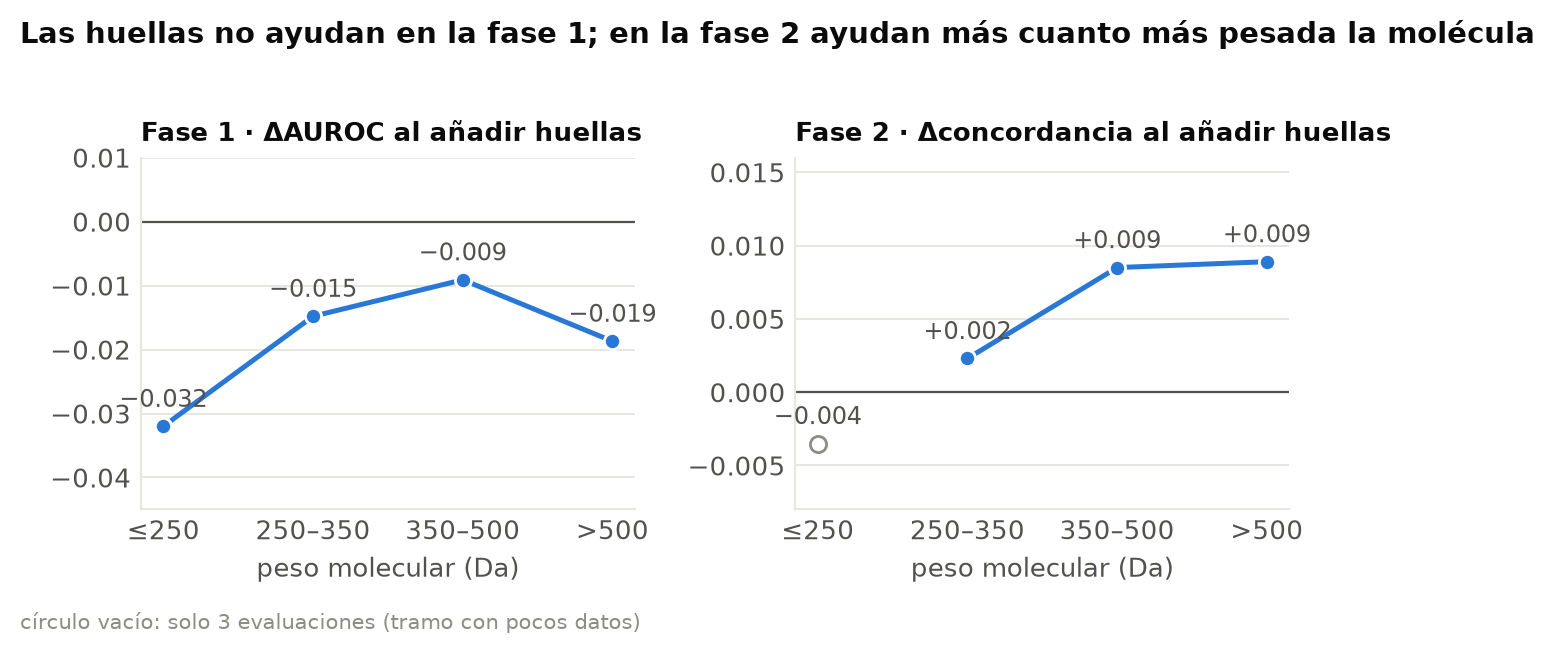
\includegraphics[width=0.9\linewidth]{figuras/f3_huellas.png}
  \caption{Cambio por añadir huellas, por tramo de peso. Magnitudes menores a 0.01 en la fase 2.}
  \label{fig:f3_huellas}
\end{figure}

\textbf{F. Los cuatro brazos del \texttt{aft} y la atribución.}

\textbf{Qué ve el modelo.} De los cuatro brazos con los mismos pliegues, ninguno supera al \texttt{aft} en NPASS: filtrar los descriptores no cambia nada que se distinga del ruido (+0.002), y \textbf{quitar los descriptores y dejar solo huellas y diana lo empeora en las 15 evaluaciones} (−0.041), aunque en el agregado empata. Esto matiza la lectura del registro (1.3) de que en la fase 2 se pueden tirar los descriptores, porque las huellas solas casi igualaban al brazo ancho: en el estrato por el que se eligió el modelo no se pueden.

\textbf{Qué pesa.} Dos métodos independientes, TreeSHAP (lee los árboles) y permutación (solo la salida), concuerdan (Spearman 0.93; 12 de sus 15 columnas más importantes son las mismas). Pesan la diana (\texttt{MAOA}, \texttt{MAOB}, \texttt{DRD2}, \texttt{LRRK2}, \texttt{BCHE}, el 15\% de la atribución) y, en la química, la complejidad topológica (\texttt{BertzCT}), la lipofilia y los halógenos. \textbf{TPSA y los donadores de hidrógeno, que dominan la permeabilidad, no dominan la potencia} (lugares 44 y 165).

\textbf{Qué pesa en la fase 1.} Los dos métodos (permutación y KernelSHAP) miran el mismo \texttt{svm\_rbf}; una versión anterior mezclaba la permutación con la impureza de un bosque, que son dos modelos, y se quitó. Coinciden en seis descriptores entre sus quince primeros (\texttt{fr\_lactam}, \texttt{NumHDonors}, \texttt{NumAliphaticCarbocycles}, \texttt{VSA\_EState3}, \texttt{fr\_Ar\_OH}, \texttt{fr\_ether}), estables entre dos muestras de compuestos; la correlación entre los dos rankings completos es 0.37. Los donadores de hidrógeno entran (puesto 4 en ambos); \textbf{TPSA no} (40 por permutación y 10 por SHAP), porque comparte información con un racimo de columnas. No se afirma ninguna estructura: son seis nombres de descriptor, no un mecanismo.

\textbf{Por subestructura.} El modelo final no usa huellas, así que se repitió el diseño con el brazo que sí (\texttt{aft\_huellas}, que no mejora en NPASS). \textbf{Con cinco repeticiones de permutación sobre las 11,248 filas, los dos métodos concuerdan según la regla declarada} (Spearman 0.577 sobre la unión de los 100 primeros, contra el 0.50 fijado de antemano, y 11 de 15 en común). Una medición previa con una repetición sobre 1,500 filas había dado 0.378 y «no concuerdan»; era ruido de la permutación, no un resultado. En la intersección hay dos subestructuras, un nitrógeno de anillo tipo piridina y un CH aromático vecino a ese nitrógeno, genéricas y frecuentes (en el 57\% y 21\% de las moléculas): indican que el modelo usa heterociclos nitrogenados, no un farmacóforo específico. \textbf{No se afirma ninguna subestructura específica.} Un límite declarado: 618 de 2,534 columnas (24.4\%, todas huellas) existen en menos de cinco pliegues y se excluyen de la intersección; ninguna estaba arriba.

\end{document}
